\documentclass[../../Raaport RayTracer]{subfiles}


\begin{document}

Pour rendre une image, le RayTracer a besoin de:
\begin{itemize}
	\item{Une résolution de rendu}
	\item{Une scène contenant les objets à rendre}
	\item{Une ou plusieures sources de lumière}
	\item{Une caméra}
	\item{Une profondeur maximale de récursion}
	\item{Un nombre de thread sur lequel le rendu sera effectué}
\end{itemize}
La résolution de rendu est fixe et est donnée au constructeur du RayTracer. La scène est les sources de lumière sont, quant à elles, dynamiques. La scène peut très bien être modifiée pendant le rendu et le RayTracer rendra les nouvelles images en conséquence.

\begin{figure}[h!]
	\adjustbox{center}{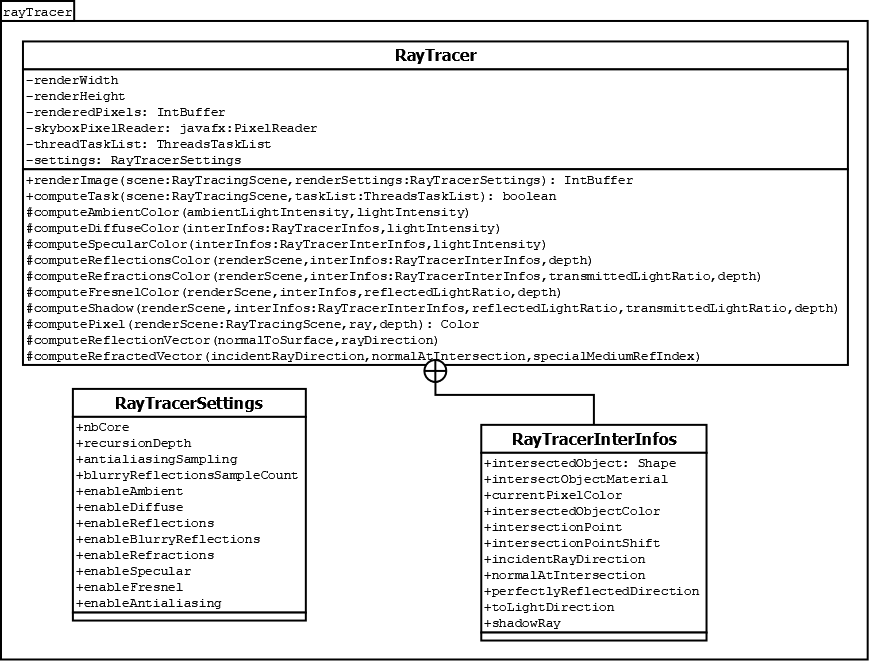
\includegraphics[width=\textwidth]{diagrammes/diagramme_RayTracer.png}}
	
	\caption{Diagramme de la classe RayTracer et de ses principales méthodes}
	\label{diagrammeRayTracer}
\end{figure}
\FloatBarrier

\begin{figure}[h!]
	\adjustbox{center}{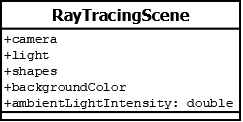
\includegraphics[width=0.52\textwidth]{diagrammes/classe_RayTracingScene.png}}
	
	\caption{Diagramme de la classe RayTracingScene contenant les informations de la scène}
	\label{diagrammeRayTracingScene}
\end{figure}
\FloatBarrier

La classe Camera, l'interface Light et la classe RayTracingScene s'organisent toutes dans le package scene:

\begin{figure}[h!]
	\adjustbox{center}{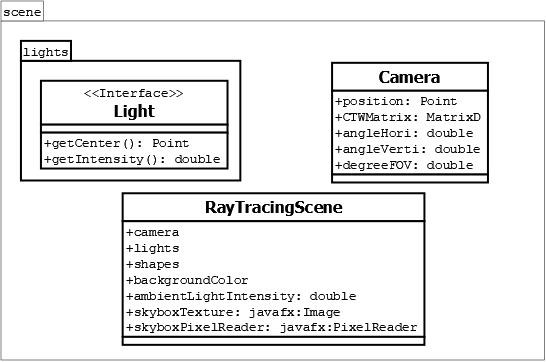
\includegraphics[width=0.75\textwidth]{diagrammes/package_scene.png}}
	
	\caption{Diagramme du package scene}
	\label{diagrammePackageScene}
\end{figure}
\FloatBarrier


\end{document}